\documentclass{../source/Experiment}

\major{信息工程}
\name{姚桂涛}
\title{振荡器与 FM \& FSK 调制}
\expname{振荡器与 FM \& FSK 调制}
\stuid{3190102932}
\college{信息与电子工程学院}
\date{\today}
\lab{东4-319}
\course{通信原理实验}
\instructor{金向东、龚淑君}
\grades{}
\exptype{验证性实验}
\partner{叶慷鹏}
\begin{document}
\makecover
\makeheader
    \section{实验目的和要求}
    (1) 掌握 LC 振荡器、晶体振荡器和压控振荡器的工作原理和电路结构

    (2) 掌握压控振荡器实现调频的方法

    (3) 对电路主要参数进行测量分析


    \section{实验原理}
    振荡器是一种不需要外部激励,就能将直流电源ᨀ供的功率
    转换成具有一定频率和振幅的信号输出的装置。振荡器一般
    由晶体管、场效应管等有源器件和具有选频能力的网络组
    成。按工作原理可分为反馈型和负阻型振荡器;按选频网络
    可分为LC振荡器、晶体振荡器和RC振荡器等。

        \subsection{振荡器的主要性能指标}

        (1) 相位噪声
        
        相位噪声和抖动是对同一种现象的两种不同定量方式。
        在振荡器的输出信号中,噪声的
        产生主要来自于晶体管及外围电路,由于振荡器为非线
        性组件,所以噪声的电压及电流会随
        时受振荡器的调变而产生。振荡器相位噪声的优劣,代
        表着振荡器的输出信号纯度是否良好。
        对于一个振荡器来说,如果没有相位噪声,振荡器的整个功率都集中在振荡频率处。
        \begin{figure}[H]
            \centering
            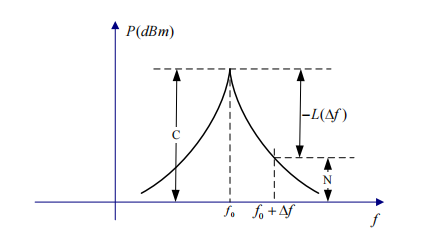
\includegraphics[width = 0.5\textwidth]{lab3/1.png}
            \caption{相位噪声示意图}    
        \end{figure}
        
        (2) 谐波失真
        
        由于振荡器存在非线性,产生的振荡信号也就存在高次
        谐波。我们用震荡信号的各高次谐波分量与基波分量的
        比值来度量谐波失真

        (3) 压控振荡器的其他性能指标

        压控振荡器的性能指标主要有:自由振荡频率,频率变
        化范围,线性度,压控灵敏度等。

        压控特性可由下面的式子表示:

        $f = f_0 + A_0v_c$


        其中, $f_0$是不加控制电压时压控振荡器的自由振
        荡频率, $A_0 $是压控灵敏度。振荡器受电压控制,
        输出频率的最大值与最小值之间的范围即为振荡器的频
        率变化范围。

        \subsection{反馈型振荡器的工作原理}
        \begin{figure}[H]
            \centering
            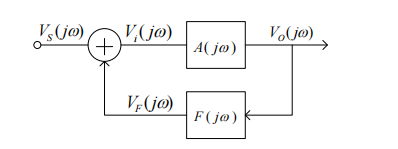
\includegraphics[width = 0.5\textwidth]{lab3/2.png}
            \caption{振荡器原理框图}    
        \end{figure}
反馈放大器的增益为:
$$
A_{f}(j \omega)=\frac{A(j \omega)}{1-A(j \omega) F(j \omega)}
$$
反馈振荡器的环路增益为:
$$
T(j \omega)=A(j \omega) F(j \omega)
$$
由以上公式可知, 若环路增益等于 1 , 那么整
个反馈放大器的增益趋于无穷大, 也就是即 使
没有外加信号, 电路也会有输出。因此, 电路自
激振荡的条件就是环路增益为 1 , 这称为振 荡
器的平衡条件, 即:
$$
T(j \omega)=A(j \omega) F(j \omega)=1
$$
其中, $|T(j \omega)|=1$ 称为振幅平衡条件; $\varphi_{T}=\varphi_{A}+\varphi_{F}=2 n \pi, n=0,1,2, \cdots$ 称为相位平衡 条件。
振荡器在平衡条件下的输出, 是在接通电源瞬间
产生的突变电流以及电路内的各种噪 声经过放
大器放大、选频、再反馈、不断增幅产生的。为
了保证在震荡初期, 振荡器的输出 信号幅度能
不断增长, 必须满足起振条件:
$$
T(j \omega)=A(j \omega) F(j \omega)>1
$$

振荡器在平衡状态时外部干扰使输
环路增益 $T$ 随 $V_{i}$ 的变化率越大, 振幅稳定性就越好。振荡器的相位稳定条件就是振荡器的频 率稳定条件。当外部干扰使振荡器的频率 $\omega$ 增大时, 则要求 $\varphi_{T}$ 减小; $\omega$ 减小, 则要求 $\varphi_{T}$ 增 大。因此频率稳定条件为: $\left.\frac{\partial \varphi_{T}}{\partial \omega}\right|_{\text {平衡点 }}<0$ 。相频特性的斜率越陡, 振荡器的频率稳定性就越好。

        \subsection{LC三点式振荡器}

        三点式振荡器采用LC振荡回路部分接入的形式,有电感
        三点式振荡器,电容三点式振荡器,改进型的电容三点
        式振荡器。

        电容三点式振荡器电路如下:
        \begin{figure}[H]
            \centering
            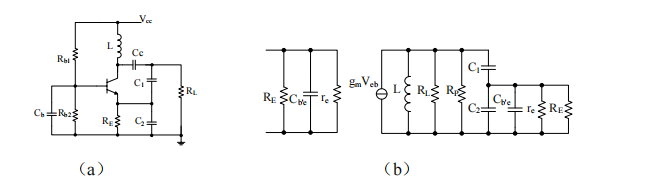
\includegraphics[width = 0.5\textwidth]{lab3/3.png}
            \caption{电容三点式振荡器电路和交流等效电路}    
        \end{figure}
        环路增益为:

        $$
        T(j\omega) = AF = \frac{g_m}{g_L' + P_{eb}^2g_i}P_{eb}
        $$

        振荡频率为:

        $$
        f = \frac{1}{2}\sqrt{\frac{1}{LC} + \frac{g_ig_L'}{C_1C_2'}}
        $$

        改进后的克拉泼振荡电路如下:
        \begin{figure}[H]
            \centering
            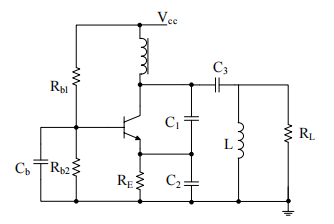
\includegraphics[width = 0.5\textwidth]{lab3/4.png}
            \caption{克拉泼振荡电路}    
        \end{figure}
        振荡频率为:

        $$
        f = \frac{1}{2\pi\sqrt{LC_3}}
        $$

        改进后的西勒振荡电路如下:
        \begin{figure}[H]
            \centering
            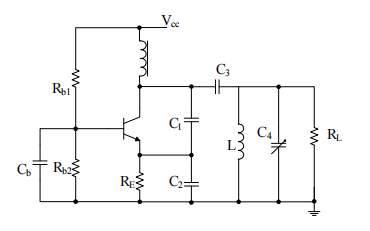
\includegraphics[width = 0.5\textwidth]{lab3/5.png}
            \caption{西勒振荡电路}    
        \end{figure}
        振荡频率为:

        $$
        f = \frac{1}{2\pi\sqrt{L(C_3+C_4)}}
        $$


        \subsection{晶体式振荡器}
        石英晶体的等效电路如下图所示。
        \begin{figure}[H]
            \centering
            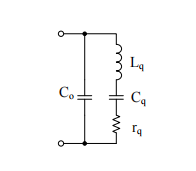
\includegraphics[width = 0.5\textwidth]{lab3/6.png}
            \caption{石英晶体的等效电路}    
        \end{figure}
        
        
        石英晶体的振荡频率
        由石英晶体和负载电容$\rm C_L$(电路中等效为与晶
        体并联的电容)确定,可以通过改变$\rm C_L$的值来
        微调振荡频率,但调节范围很小。晶体振荡器的频率

        $$
        f = \frac{1}{2\pi\sqrt{L_q\frac{C_q(C_o+C_L)}{C_q+(C_o+C_L)}}}
        $$

        \subsection{压控振荡器}
    振荡器频率由电压控制,作线性变化,即为压控振荡器。通
    常,将变容二极管作为可变电容,接入LC振荡器中,构成压
    控振荡器。变容二极管在反向偏置条件下,它的势垒电容随
    外加电压变化,电容$C_j = C_o/(1+\mu/\mu_{\varphi}
    )$,$C_o$ 是变容二极管偏置为零时的结电容, 
    $\mu_\varphi$是变容二极管PN结的势垒电位差,
    $\gamma$是结电容变化指数,与制造工艺有关。

        \subsection{FM\_FSK调制}
        FM调频产生的方法主要有两种,直接调频和间接调频。直接调频就是调制信号直接作用
        于振荡器,使振荡频率随调制信号变化。对于LC振荡电路,由调制信号控制其中的一个电抗
        元件,使它随调制信号变化,则振荡频率将受控与调制信号,达到调频的目的。在高频电路
        中,经常由变容二极管来实现。

        假设加在变容二极管上的调制信号电压
        为 $u_{\Omega}(t)=U_{\Omega} 
        \cos \Omega t$, 静态工作点上的电
        压为 $U_{Q}$, 则变容二极管上的结
        电容为 $C_{j}=C_{Q}(1+m \cos 
        \Omega t)^{-\gamma}$ 。其中, 
        $C_{Q}=C_{o} /\left(1+U_{Q} / 
        u_{\varphi}\right)^{\gamma}$, 
        为静态 工作点上的结电容。 $m=U_
        {\Omega} /\left(U_{\Omega}+u_
        {\varphi}\right)$, 为电容调制
        度, 即结电容受调制信号影响的程
        度。 调制信号的变化导致结电容的变
        化, 从而影响振荡器频率的变化, 实
        现调频。
       
        线性调制频偏为 $A_{1} m \omega_
        {c} \cos \Omega t$, 相 移为频偏
        的积分, 等于 $\mid A_{1} m 
        \omega_{c} \frac{\sin \Omega t}{\Omega}$ 。最大相移就是调制度, 等于 $\frac{A_{1} m \omega_{c}}{\Omega}$ 。
    \section{实验电路分析}
    \begin{figure}[H]
        \centering
        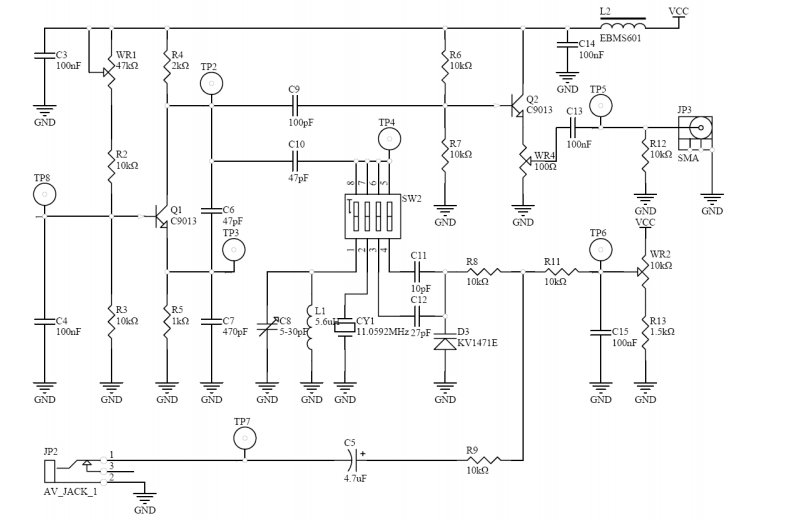
\includegraphics[width = 0.5\textwidth]{lab3/7.png}
        \caption{振荡器与 FM\_FSK 调制电路}    
    \end{figure}
    实验电路如上图所示。SW2为振荡器选择开关,将SW2设成
    “1000”,就构成了一个改进型的电容三点式振荡器,通过调
    节C8,可以改变振荡频率;将SW2设成“0100”,电容三点式
    振荡器中的电感用石英晶体代替,就构成并联型石英晶体振
    荡电路,电容C6、C7、C10、C8构成的等效电容称为晶体的
    负载电容CL。

    将SW2的第一位开关接通接通,在构成改进型电容三点式振
    荡器的基础上,再接通第三位或者第四位开关(即设为
    “1010”或“1001”),将变容二极管接入电路中,就构成压
    控振荡器。改变滑动变阻器WR2的阻值,变容二极管上的直
    流电压也随之改变,就可以改变振荡频率。

    在压控振荡电路连接方式下,音频调制信号可由JP2端口接
    入,与来自WR2的静态电压通过电阻网路叠加后加到变容二
    极管,则振荡频率将受控于调制信号,达到调频的目的。若
    调制信号是正弦信号,则为FM调制;若调制信号是脉冲信
    号,则为FSK调制。

    实验电路中,振荡电路的静态工作点将影响电路的工作状
    态,可通过WR1调整。Q2及外围的电阻器件构成了跟随电
    路,降低了振荡电路的输出阻抗,同时避免负载对于振荡电
    路的影响。通过调节WR4还可调整输出信号幅度。


    \section{实验设备}
        \begin{enumerate}
            \item 实验办No01 \, 1块
            \item 信号源1台
            \item 双踪示波器1台
            \item 频谱分析仪(含TG)1台
            \item 万用表1台
        \end{enumerate}
        
    \section{实验数据与结果分析}
        \subsection{振荡器相位噪声的测量}

        将SW2设置为“0100”,构成晶体振荡器电路。用示波器
        观察TP5端信号波形,调节电位器WR1,使振荡器起振
        并使输出信号幅度最大,且波形无明显失真。

        设定频谱分析仪中心频率为12.000MHz,扫᧿宽度为
        100KHz,分辨率带宽为1kHz,参考电平为10dBm;为
        使显示波形稳定,可采用功率平均显示方式:【Trace】【迹线类型】【功率平均】。

        采用峰值搜索功能键【Peak】读取总功率(C),再用
        差值光标方法读取峰值差值:【Mark】、【差值】
        【20】【kHz】,读取距离中心频率20kHz处噪声功率
        与峰值功率的差值(N-C)。将测得的数值代入式3.3.
        3,即可计算得到相位噪声。
 
        \begin{figure}[H]
            \centering
            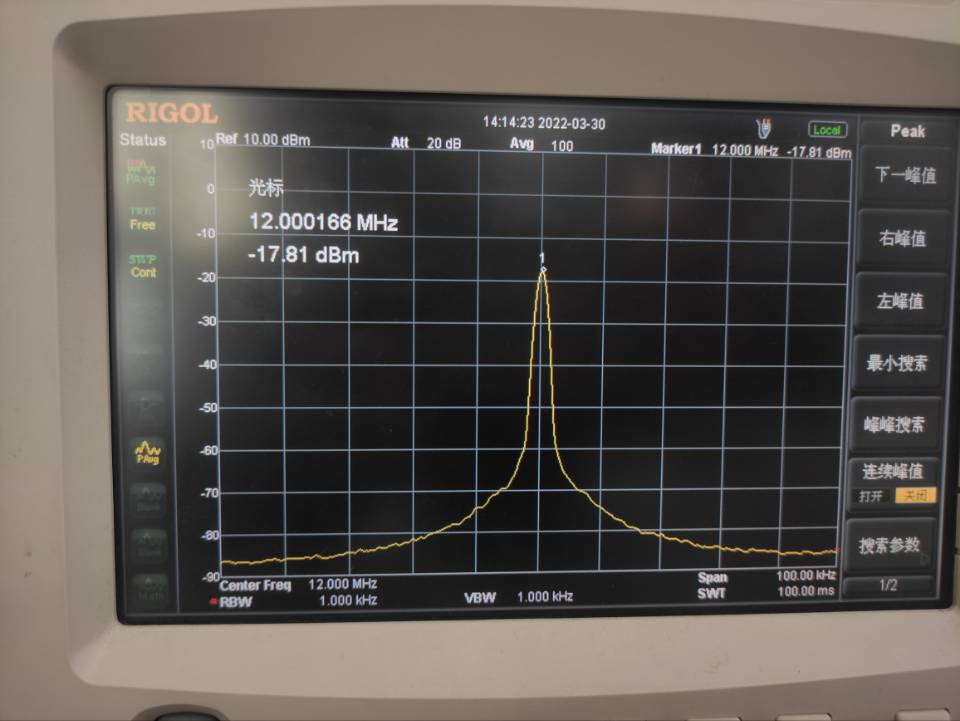
\includegraphics[width = 0.5\textwidth]{lab3/1.jpg}
            \caption{总功率C}    
        \end{figure}
        从图中可以看出,总功率C为-17.81dBm。
        \begin{figure}[H]
            \centering
            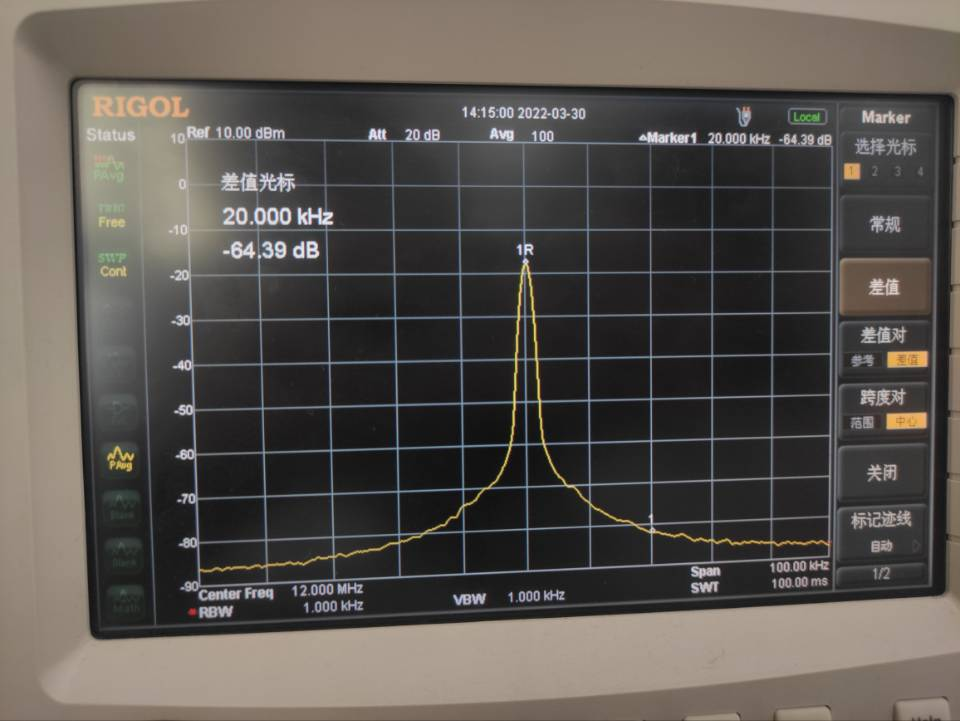
\includegraphics[width = 0.5\textwidth]{lab3/2.jpg}
            \caption{离中心频率20kHz处噪声功率与峰值功率的差值}    
        \end{figure}
        读出差值N-C等于-64.2dB。
        
        带入公式$$L(\Delta f)=N(R B W)-C-10 \log (1.2 \times R B W)$$
        
        可得$L(\Delta f)$=-94.9918dB,计算值即为相位噪声大小。

        \subsection{谐波失真的测量}
        设定频谱分析仪中心频率为 12MHz,扫宽为 10MHz;按【Peak】搜索峰值;按【Meas】
        【测量功能】【下页】进入测量功能并选取【谐波失真】;读取基波及 2 至 4 次谐波幅度值。
        计算谐波失真数值。
        \begin{figure}[H]
            \centering
            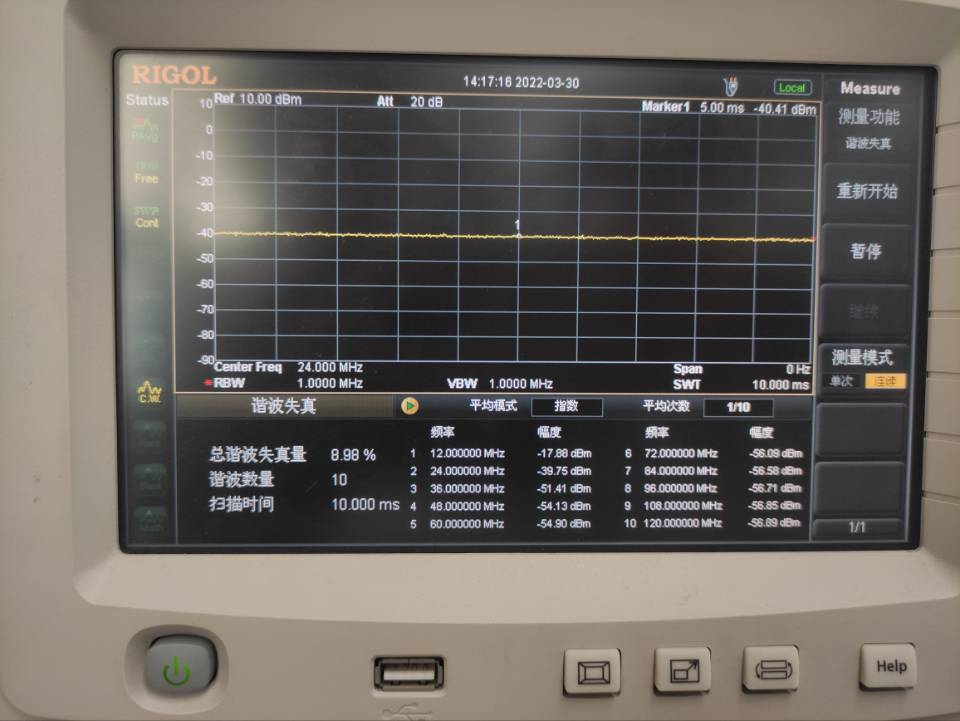
\includegraphics[width = 0.5\textwidth]{lab3/3.jpg}
            \caption{测量并选取谐波失真}    
        \end{figure}

        从上图中可以读出,基波幅度为-17.88dBm,2次谐波幅度为-39.75dBm,3次谐波幅度为-51.41dBm,4次谐波幅度为-54.13dBm。

        因此计算得2次谐波失真为-21.87dB,3次谐波失真为-33.53dB,4次谐波失真为-36.25dB。

        可以看出谐波次数越高,失真情况越大。

        \subsection{压控振荡器频率范围及压控增益的测量}

        将SW2设置为“1010”或“1001”,构成压控振荡器电
        路。调节电位器WR2,改变加在变容管D3上的电压(可
        在测试点TP6测得压控电压),用示波器或频谱分析仪
        观察振荡器输出信号的频率变化。分别记录压控电压为
        1V和4V时的振荡频率记为压控范围,计算压控增益。
        \begin{figure}[H]
            \centering
            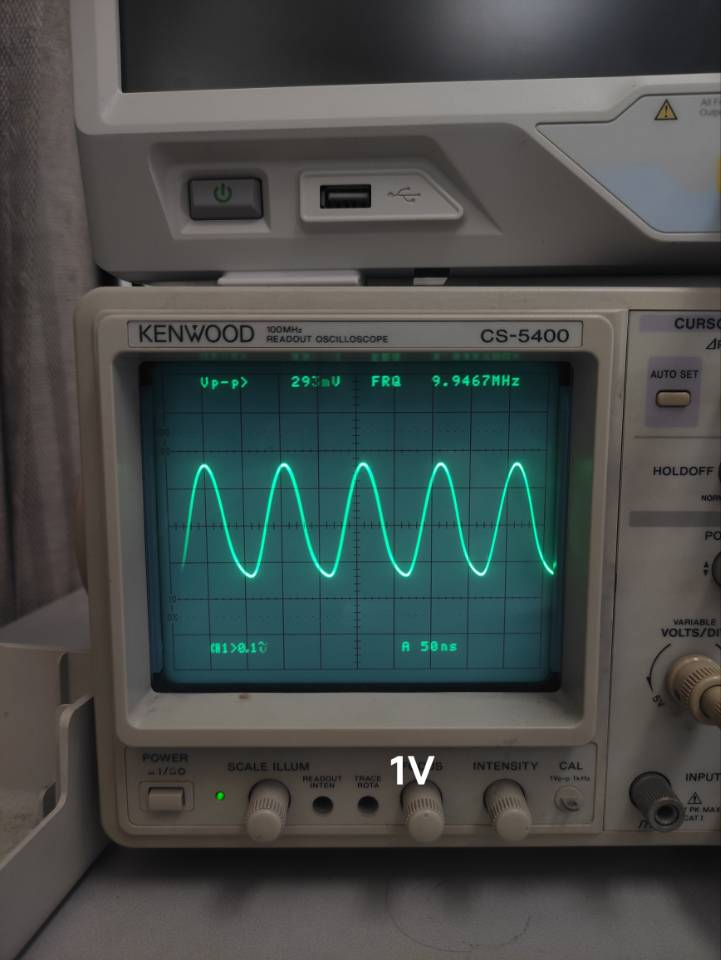
\includegraphics[width = 0.5\textwidth]{lab3/4.jpg}
            \caption{1V时得振荡频率}    
        \end{figure}
        从上图中可以读出压控电压为1V时得振荡频率为9.946MHz。

        \begin{figure}[H]
            \centering
            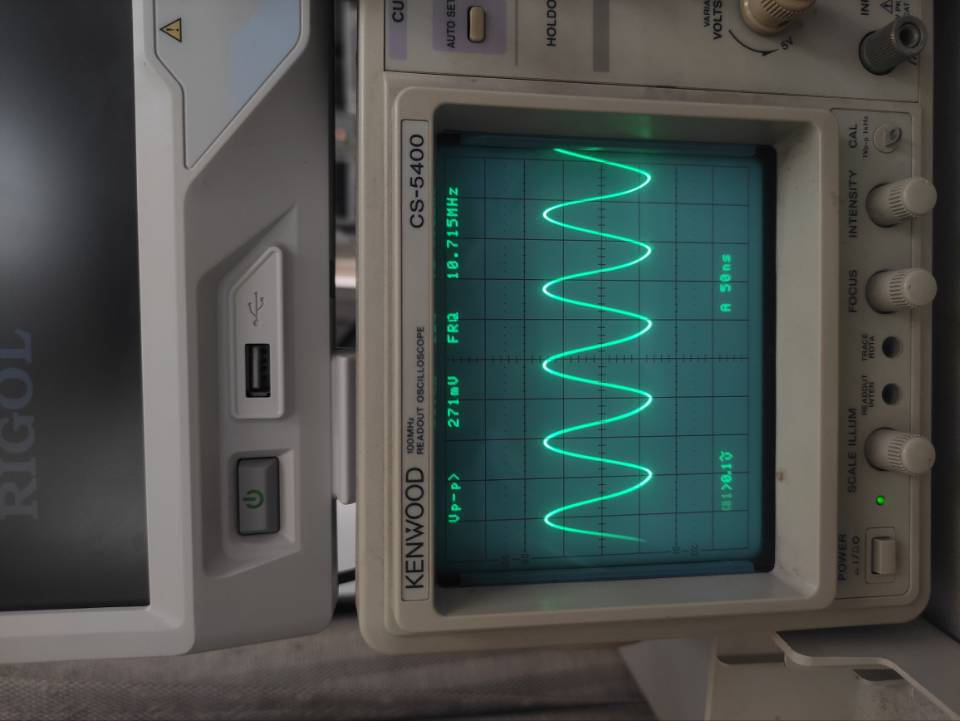
\includegraphics[width = 0.5\textwidth,angle=270]{5.jpg}
            \caption{4V时得振荡频率}    
        \end{figure}
        压控电压为4V时得振荡频率为10.715MHz。

        因此压控增益A=$\frac{\delta f}{\delta v}$=(10.715-9.946)/(4-1)=0.255MHz/V.
        
        \subsection{FM\_FSK 调制频偏的测量}

        频偏为调制信号频谱中肩峰处频率值与中心频率的差值。测量步骤如下:
        
        通过WR2调整变容二极管的静态工作点,调整到TP6的
        直流电压为2.5V左右;将高频信号源与电路板JP2端相
        连,输入频率为1KHz,幅度为-10dBm的正弦波信号;
        设定频谱分析仪的中心频率为10.7MHz,扫频宽度为
        500kHz,分辨率带宽为1KHz,视分比为0.1;采用差值
        光标方法测量输入信号为-10dBm对应的频偏量;改变
        输入信号的大小在-10dBm至0dBm之间变化,观察调制
        频偏的变化情况。
        \begin{figure}[H]
            \centering
            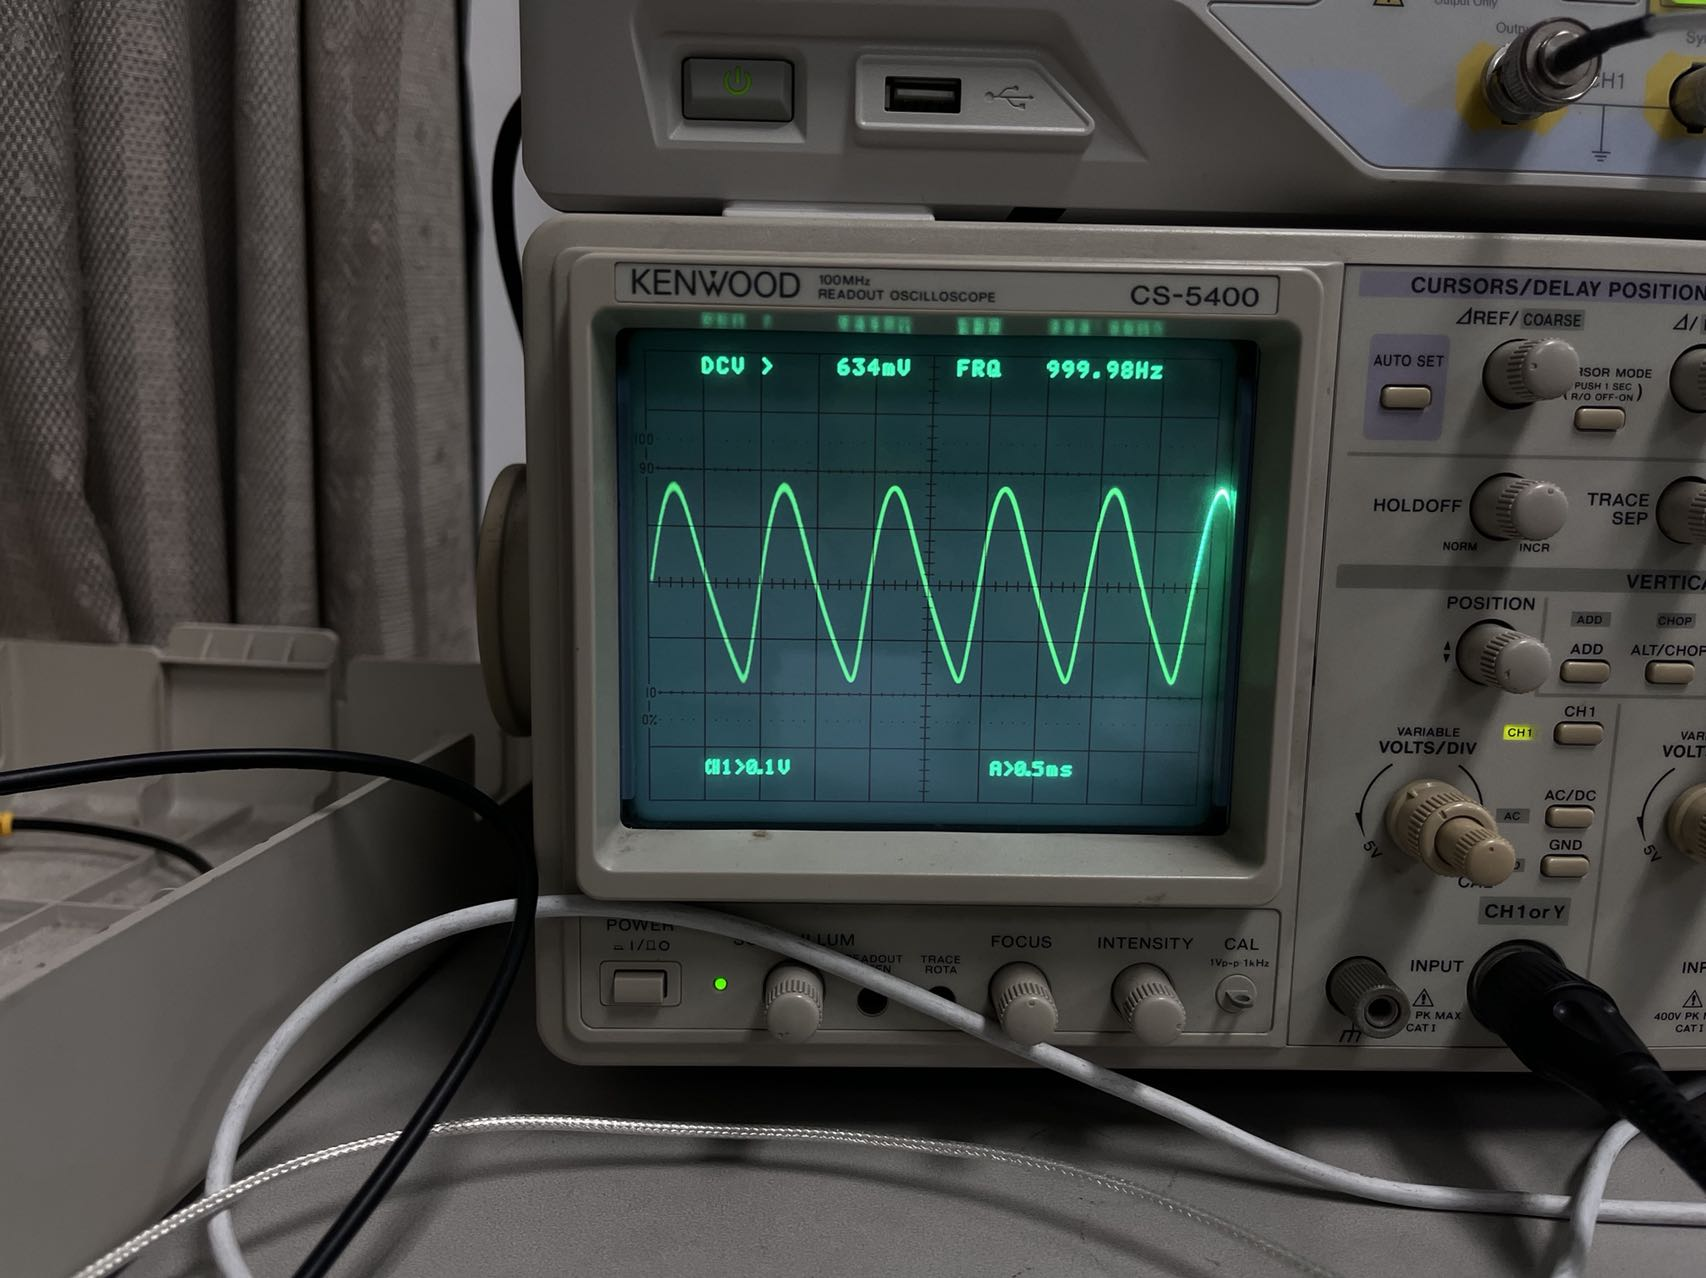
\includegraphics[width = 0.5\textwidth,angle=270]{6.jpg}
            \caption{FM\_FSK 调制频偏的测量示意图}    
        \end{figure}
        
        输入信号与频偏对应关系的表格如下:
        \begin{table}[H]
            \centering
            \begin{tabular}{|l|l|}
            \hline
            输入信号幅度/dBm & 频偏量/kHz \\ \hline
            -10        & 20.417  \\ \hline
            -8         & 26.665  \\ \hline
            -6         & 33.334  \\ \hline
            -4         & 42.917  \\ \hline
            -2         & 54.167  \\ \hline
            0          & 67.917  \\ \hline
            \end{tabular}
            \end{table}
        可以看到,随着输入信号幅度增大,FM调制的频偏也在增大。

        将信号源输出的波形设定为方波,此
        时可视为FSK调试,观察调制信号频谱有何变化。
        \begin{figure}[H]
            \centering
            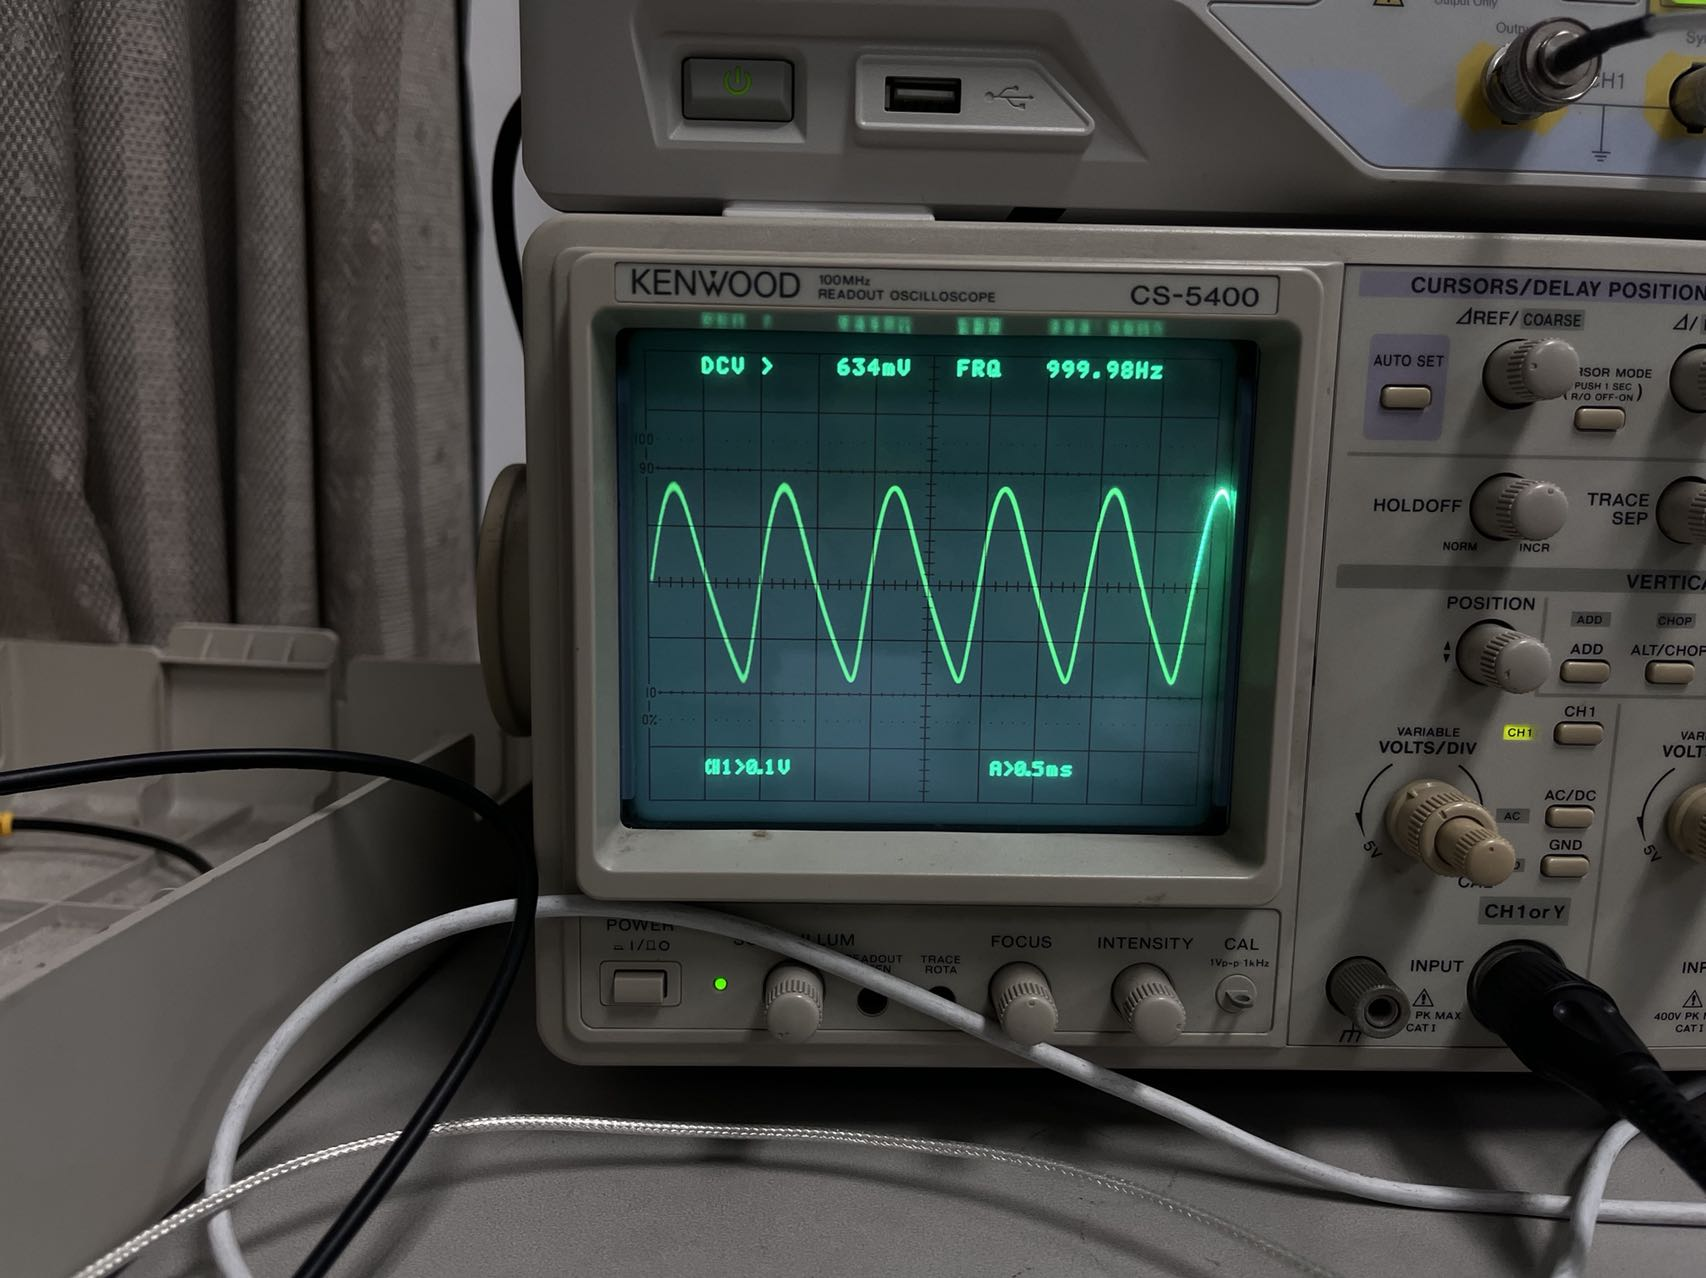
\includegraphics[width = 0.5\textwidth,angle=270]{6.jpg}
            \caption{方波FSK调试}    
        \end{figure}

        可以看到FSK调制时,频偏量变小。

    \section{思考题}
	    \subsection{为什么振荡器起振后的直流工作点电流不同于起振前的静态工作点电流?}
        电路起振前,其工作状态是固定的,所以电流一般为定值。电路起振后,其工作状态在导通和截止之间不停的转换,其电流会和起振前不同
        
        电路起振前,工作状态固定,电流为定值;起振后,工作状态在导通截止之间转换,电流也随之变化。
        \subsection{为什么反馈系数要选取 F=1/2-1/8,过大,过小有什么不好?}

        太大会导致品质因数Q值降低;太小不容易满足振幅起振条件。
        \subsection{对于 LC 电路,为什么当静态电流发生变化时,其振荡频率会发生变化?}
        因为电容漏电不等于0,致使静态电流越大,温升越不可忽视,对电容量影响越大,所以其振荡频率会发生变化。
        
\end{document}